%************************************************
% IMPLEMENTATION
%************************************************

\chapter{Implementation} \label{chap: implementation}

\paragraph{} \textit{In this chapter we present the tools that have been used for the implementation of the project, some details about the data, the data preprocessing procedure, a description of the models' configurations and experiments conducted and the produced results.}


%----------------------------------------------------------------
% Tools
%----------------------------------------------------------------

\section{Tools} \label{sec: tools}
\paragraph{} All the computation for this project has been conducted on a university server equipped with Ubuntu SMP version 16.04.1 and a NVIDIA TITAN Xp graphics card for the deep learning training processes. A brief description of the software tools used for the project will follow.

\paragraph{Python} \cite{python} The programming language used for this project is Python v3.6. Python is a general purpose language, known for its ease of use and understanding; however, thanks to the addition of dedicated libraries for data analysis and predictive modeling, in the last few years it has become the reference and most-used language for data science.

\paragraph{Numpy} \cite{numpy} Numpy is an extremely popular and useful library for scientific computing with Python. It allows to easily handle multidimensional data through matrix representation and to perform operation between them thanks to its broadcasting functions. Numpy has been used in all the project implementation's steps to handle and manipulate the data.

\paragraph{Pandas} \cite{pandas} Pandas is an open source library which provides efficient, flexible and easy-to-use data structures and data analysis tools for Python. Pandas is built on top of Numpy library and it is suited to handle almost any kind of data, representing them in a handy tabular form. We mainly used Pandas in order to store the results from the experiments.

\paragraph{matplotlib} \cite{matplotlib} Matplotlib is a 2D plotting library and it represents one of the most common visualization tools for Python. Its \texttt{pyplot} module provides a MATLAB-like functional interface and a wide degree of customization of the generated figures. All the plots in this thesis has been generated using matplotlib library.

\paragraph{scikit-learn} \cite{scikit-learn} Scikit-learn is a well-known, simple and efficient library for data analysis and machine learning in Python. It is open-source and is built on NumPy, SciPy, and matplotlib libraries. It provides several useful tools for data preprocessing, model selection, classification, regression, clustering and dimensionality reduction. In this project, it has been heavily used for the data preprocessing and to implement the classic machine learning models.

\paragraph{XGBoost} \cite{xgboost} XGBoost is an optimized library for distributed gradient boosting, designed to be highly efficient, flexible and portable. It implements a tree-based gradient boosting model which has been used for the gradient boosting experiments.

\paragraph{Tensorflow \& Keras} \cite{tensorflow} \cite{keras} The framework we used in order to build deep learning models is Tensorflow v2.0. Tensorflow is one of the most popular frameworks for machine learning and deep learning; it is open-source and it provides a flexible ecosystem of tools, libraries and community resources to easily build machine learning models. On top of Tensorflow, we used Keras high-level neural networks API. Keras was originally a library separated from Tensorflow, providing ready-to-use tools for fast experimentation and developing of neural networks models by running on top of TensorFlow, CNTK, or Theano. With the update to version 2.0 of Tensorflow, Keras has officially become part of Tensorflow API. We mainly used Keras library on top of Tensorflow for the implementation of deep learning models in order to generate high-level and easy-to-understand code. This choice was reasoned by the fact that this thesis project is also related to the medical field, so we tried to make the code readable also by people which are not specialized in the data scientist field.

\paragraph{Spektral} \cite{Spektral} Spektral is a Python library for graph deep learning, based on the Keras API. It provides a simple but flexible framework for creating graph neural networks (\acsp{gnn}) by making available several ready-to-use, but still highly customizable, graph-based deep learning layers. It also implements functions for the creation of the functional connectivity network from a data stream. In this project, Spektral library was used for the generation of functional connectivity graphs and for the implementation of graph-based deep learning models.


%----------------------------------------------------------------
% Data analysis
%----------------------------------------------------------------

\section{Data analysis} \label{sec: data_analysis}

\paragraph{} For this project, we were provided with 24 hours of \acs{ieeg} data generated from real measurements on a patient suffering form epilepsy. The data contains three seizures, all happening during the first three hours of recording; therefore just the data regarding the first three hours have been used in the project. The brain activity has been measured using 90 electrodes and a sampling frequency of 500 Hz, so each hour contains $1\,800\,000$ time steps of measurements.

First thing, we identified the position of the seizures in the data and their length. As already mentioned, the data contains three seizures in total, each one having a duration between $13\,000$ and $15\,000$ time steps, for a total of $42\,000$ time steps of seizure. This corresponds to 26 to 30 seconds of duration for each seizure and 84 seconds of seizure in total. Since the most important data for this project were the seizure time steps and we did not need a huge amount of non-seizure time steps, during all the project we considered only a portion of data around each one of the three seizures, obtaining $450\,000$ time steps (15 minutes) to work with between seizure and non-seizure data in total. This should give an idea of how much limited the amount of useful data was for this project.

Some basic statistical measurements have been applied to the \acs{ieeg} data in order to familiarize with its features. The measured voltage in the \acs{ieeg} vary between about $-9\,500$ and $9\,800$ \acs{uv} (microvolts), covering a range of about $19\,300$ \acs{uv}. Each electrode's signal oscillate through time with a standard deviation of around 82 \acs{uv} and the various electrodes signals cover different areas of the \acs{ieeg} voltage range based on their placement on the brain surface. In Figure \ref{fig:plot_seizures} the plots of the \acs{ieeg} around the three seizures is shown. The start and end times of the seizures in each plot are indicated by red vertical lines.
\todo{Change following 3 iEEGs to high-quality corresponding images}
\newpage
\begin{figure}[H]
    \centering
    \begin{subfigure}[t]{0.7\textwidth}
		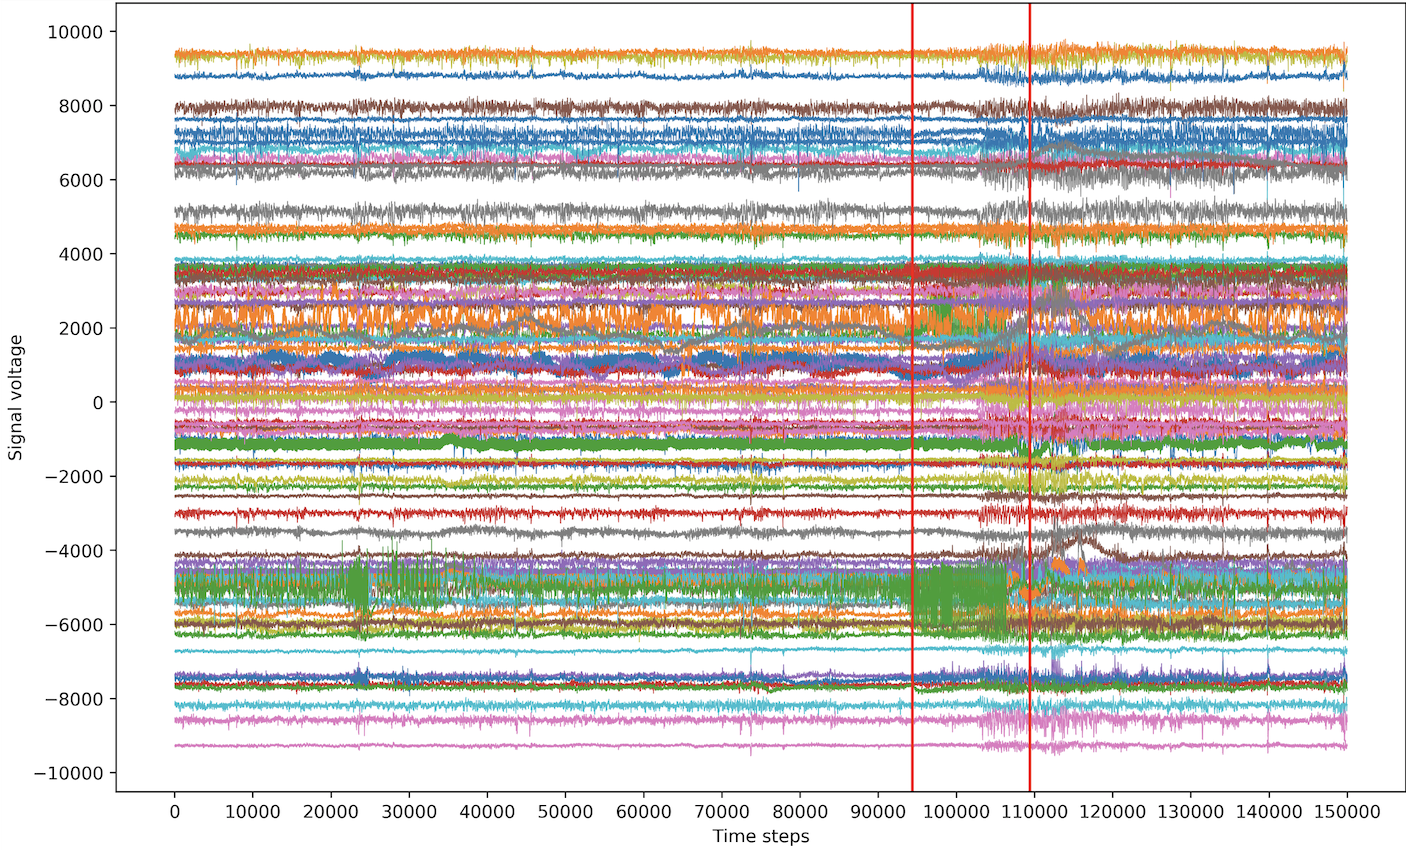
\includegraphics[width=1\textwidth]{plot_seizure1_lowquality}
        \caption{First epileptic seizure}
        \label{fig:plot_seizure1}
	\end{subfigure}
	~
	\begin{subfigure}[t]{0.7\textwidth}
		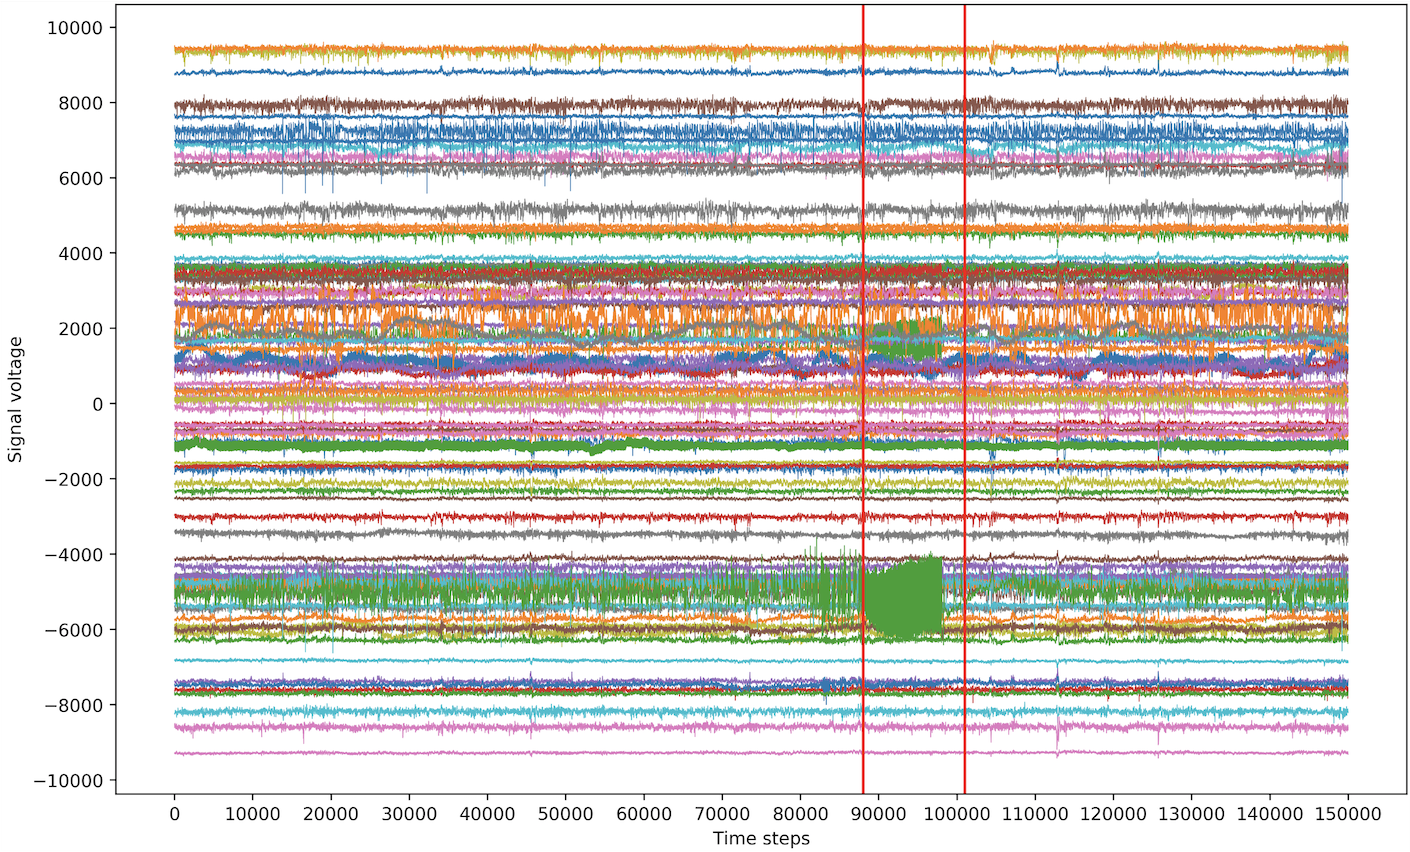
\includegraphics[width=1\textwidth]{plot_seizure2_lowquality}
        \caption{Second epileptic seizure}
        \label{fig:plot_seizure2}
    \end{subfigure}
    ~
    \begin{subfigure}[t]{0.7\textwidth}
		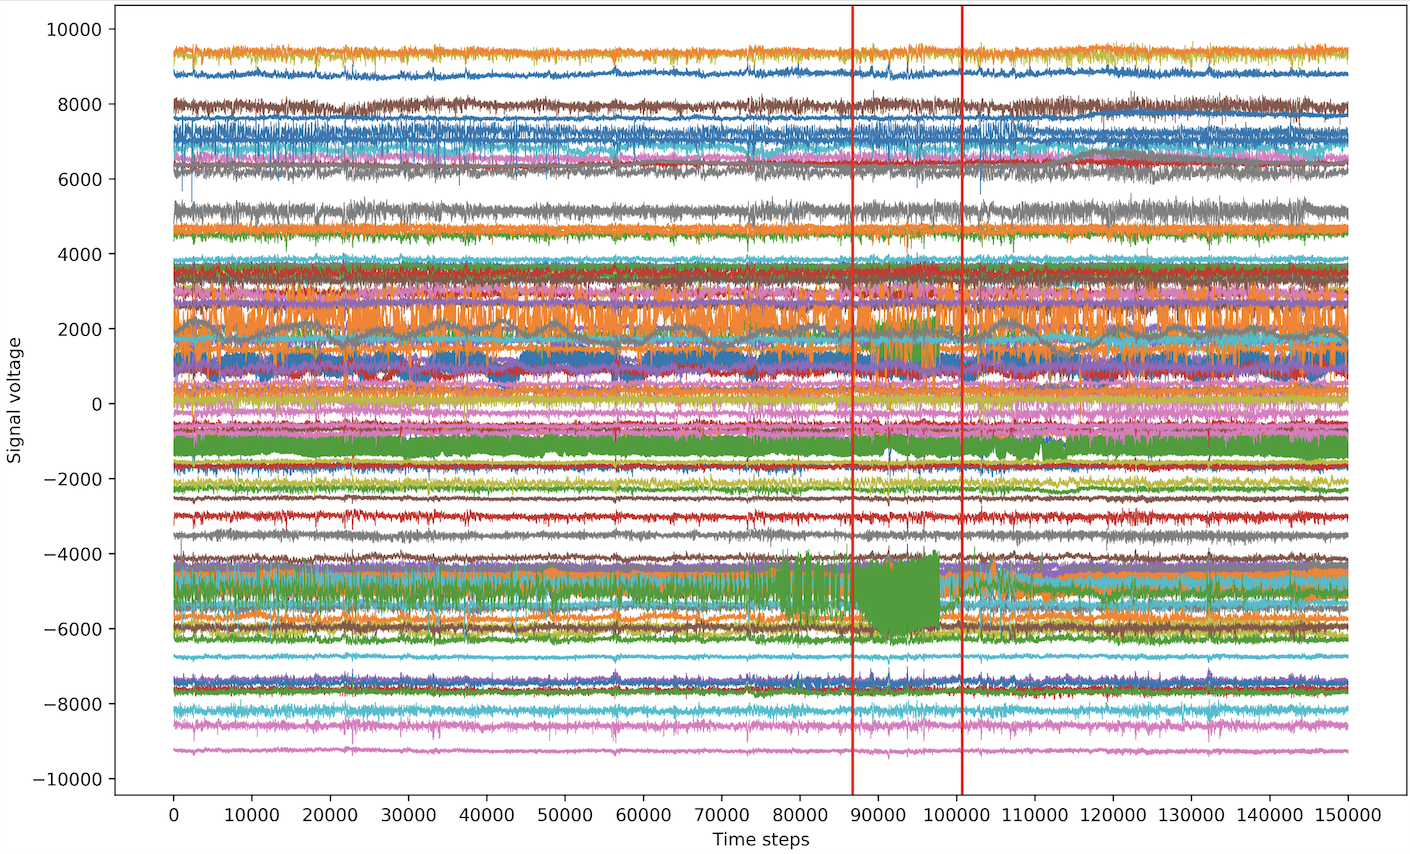
\includegraphics[width=1\textwidth]{plot_seizure3_lowquality}
        \caption{Third epileptic seizure}
        \label{fig:plot_seizure3}
	\end{subfigure}
    \caption{Plots of the \acs{ieeg} around the three epileptic seizures (we suggest to zoom-in the figures in the pdf file)}
    \label{fig:plot_seizures}
\end{figure}
% \begin{figure}[H]
%     \centering
%     \begin{subfigure}[t]{0.7\textwidth}
% 		\includegraphics[width=1\textwidth]{plot_seizure1}
%         \caption{First epileptic seizure}
%         \label{fig:plot_seizure1}
% 	\end{subfigure}
% 	~
% 	\begin{subfigure}[t]{0.7\textwidth}
% 		\includegraphics[width=1\textwidth]{plot_seizure2}
%         \caption{Second epileptic seizure}
%         \label{fig:plot_seizure2}
%     \end{subfigure}
%     ~
%     \begin{subfigure}[t]{0.7\textwidth}
% 		\includegraphics[width=1\textwidth]{plot_seizure3}
%         \caption{Third epileptic seizure}
%         \label{fig:plot_seizure3}
% 	\end{subfigure}
%     \caption{Plots of the \acs{ieeg} around the three epileptic seizures (we suggest to zoom-in the figures in the pdf file)}
%     \label{fig:plot_seizures}
% \end{figure}
\newpage

Looking at Figure \ref{fig:plot_seizures}, it seems like the \acsp{ieeg} is not able to explicitly show the presence of a seizure, since the dynamic of the electrodes signals does not seem to undergo a big change in correspondence of the beginning of a seizure. This behaviour suggests that the seizure could not be directly represented by the dynamic of the signals, but it could be represented by the non-linear relations between the electrodes signal's dynamic through time.

The amount of positive time steps, that are the ones inside the seizure portions, corresponds only to the $9.3$\% of the data, with the remaining $90.7$\% of data being negative time steps; therefore we are dealing with very unbalanced data (see Figure \ref{fig:hist_classes}). The extreme unbalance of the data, together with the severe restriction in the amount of data, make this dataset very difficult to work with, but at the same time very similar to a real-world scenario.
\begin{figure}[htbp]
    \centering
    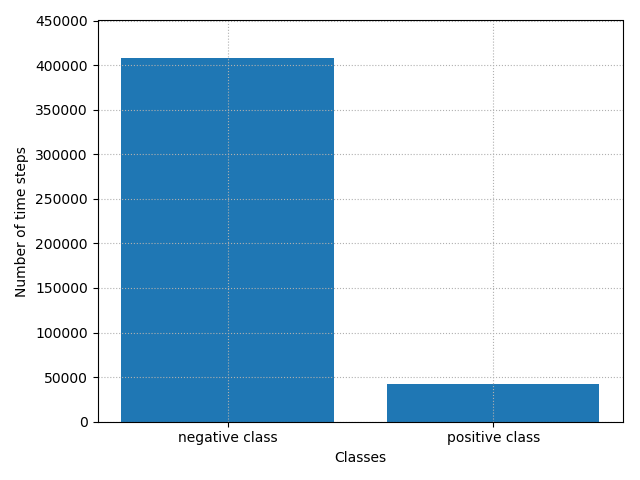
\includegraphics[width=0.6\textwidth]{hist_classes}
    \caption{Histogram of the number of time step for each class}
    \label{fig:hist_classes}
\end{figure}

In order to have an idea of the linear relation between electrodes values, we computed the Pearson correlation coefficient on two sequences of 5 seconds each, one of negative time steps and the other of positive time steps. In Figure \ref{fig:corr_heatmaps} we show the related correlation heatmaps. As you can see from the figures, the correlation heatmap related to the positive time steps reveals a higher linear relation between electrodes values if compared to the correlation heatmap related to the negative time steps. The correlation heatmaps, however, present only the linear relations between data, while we believe that there are hidden non-linear relation between electrodes signal through time which could be crucial for the identification of epileptic seizures.

\begin{figure}[htbp]
    \centering
    \begin{subfigure}[t]{0.49\textwidth}
		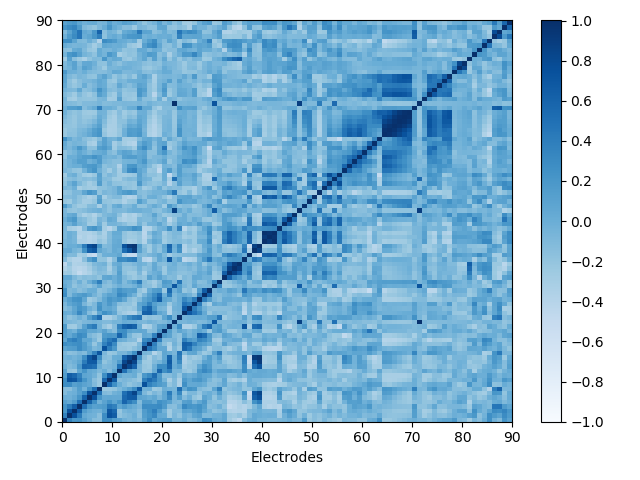
\includegraphics[width=1\textwidth]{corr_nonseizure}
        \caption{Correlation heatmap of 5 seconds of negative time steps}
        \label{fig:corr_nonseizure}
	\end{subfigure}%
	~
	\begin{subfigure}[t]{0.49\textwidth}
		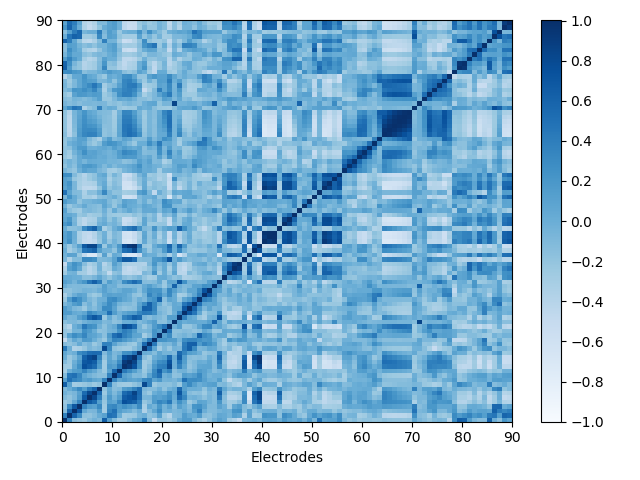
\includegraphics[width=1\textwidth]{corr_seizure}
        \caption{Correlation heatmap of 5 seconds of positive time steps}
        \label{fig:corr_seizure}
    \end{subfigure}
    \caption{Comparison of correlation heatmaps related to negative and positive time steps}
    \label{fig:corr_heatmaps}
\end{figure}

To have another confirmation of the presence of some linear relation between electrodes signals, we computed the standard deviation of the oscillation of each electrode, but this time we computed the mean of the standard deviation both over the negative time steps and over the positive ones. The average standard deviation of the oscillation of each electrode over the negative time steps was around 80 \acs{uv}, while the one over the positive time steps was around 93 \acs{uv}. This shows that, during an epileptic seizure, electrodes signals tends to have wider fluctuation margins, but the difference from the standard fluctuation margins does not seems to be enough to identify a seizure.

%----------------------------------------------------------------
% Data preprocessing
%----------------------------------------------------------------

\section{Data preprocessing} \label{sec: data_preprocessing}
\paragraph{} Once we familiarized with the dataset, we preprocessed it in order to shape it to the right form to be the input of machine learning and deep learning models for the different prediction tasks. As already mentioned in Section \ref{sec: step_data_preprocessing}, we divided the data in a training set and a test set, using two seizures' data in the training set and the remaining seizure's data in the test set. We sacrificed the validation set for lack of data. The data was prepared to be used by different models for the three prediction tasks described in Section \ref{sec: problem_definition}. Depending on the model and on the task at hand, a sample could represent a time step, a sequence of samples or a sequence of graphs.

\subsection{Time steps as samples}
\paragraph{} This data configuration has been used only for the problem case of detection on a time step; therefore it as been used as input to random forest, gradient boosting, \acs{svm} and dense neural network. In order to prepare data with each time step representing a sample, no additional operations where required, since the dataset was already provided as a big sequence of time step - target couples. Since \acsp{svm} and neural networks are sensible to the scaling of the data, in those cases a \texttt{StandardScaler} from scikit-learn library has been added. The \texttt{StandardScaler} standardize the features of a sample such that the data distribution will have a mean value equal to 0 and a standard deviation value equal to 1. The standardization is computed as:
\begin{align}
    z=\frac{x-\mu}{\sigma} \qquad\qquad \text{with}\qquad &\mu=\frac{1}{N} \sum_{i=1}^{N}\left(x_{i}\right)\\
                                        \text{and}\qquad &\sigma=\sqrt{\frac{1}{N} \sum_{i=1}^{N}\left(x_{i}-\mu\right)^{2}}
\end{align}
where $z$ is the standardized version of $x$, $\mu$ is the mean of $x$ and $\sigma$ is the standard deviation of $x$.

\subsection{Sequences of time steps as samples}
\paragraph{} This data configuration has been used for the problem cases both of detection on a sequence and of prediction on a sequence. The sequences of time steps generated has been the input to standard convolutional and 
\acs{lstm} neural networks. In order to prepare data with each sequence of time steps representing a sample, the dataset has been converted in a set of sequences with a single target associated to each sequence. To do that, we implemented a function that considers different parameters.

The \texttt{look\_back} parameter indicates the number of time steps contained in each sequence; in other words it represents the amount of time steps at which the model can look at in order to predict a target.

The \texttt{target\_steps\_ahead} parameter determines how far in the future we want the target time step of a sequence to be, starting from the position of the last time step of the sequence. This means that if we set \texttt{target\_steps\_ahead}=0, the model will use the sequence's features to predict the target associated with the last time step of the sequence, that corresponds to the problem case of detection on a sequence. Alternatively, if we set \texttt{target\_steps\_ahead}>0, the model will use the sequence's features to predict the target associated with a time step outside the sequence and in the future, that corresponds to the problem case of prediction on a sequence.

The \texttt{stride} parameter sets the size of the distance between the beginning time step of two consecutive sequences. For instance, if \texttt{stride}=1, the sequences will begin time steps at indices $i_0, i_1, i_2, i_3, ...$, while if \texttt{stride}=3, the sequences will begin with time steps at indices $i_0, i_3, i_6, i_9, ...$.

The \texttt{subsampling\_factor} parameter adds a downsampling effect to the number of sequences by keeping a factor of negative samples with respect to the positive ones. This means that if, for example, \texttt{subsampling\_factor}=5, for each positive sample we will keep only five negative samples. This is useful in order to decrease the unbalance in the data. The downsampling effect is applied only if the parameter \texttt{subsample} is set to \textit{True}.

The function we implemented to generate the sequences of time steps considers one time step index at a time, it takes the previous \texttt{look\_back} time steps to create the sequence and it looks \texttt{target\_steps\_ahead} time steps ahead to identify the target to assign to the sequence. After that, it consider the next time step index, which is \texttt{stride} time steps after the current one, and repeats the process. After having created all the sequences, the function discards some random negative sequences in order to respect the proportion between positive and negative samples given by the \texttt{subsampling\_factor}.

In order to create this data configuration, we preprocessed the data by first applying a \texttt{StandardScaler}, like in the previous case, and then using the sequence generator function both on the training set and the test set, using the same parameters for both of them. The only difference was the use of \texttt{subsample}=\textit{False} for the test set, since during the testing of the model we do not need to compensate the unbalance of the dataset.

\subsection{Sequences of graphs as samples}
\paragraph{} This data configuration has been used for the problem cases both of detection on a sequence and of prediction on a sequence. The sequences of graphs generated has been the input to graph-based convolutional and 
\acs{lstm} neural networks. In order to prepare data with each sequence of graphs representing a sample, the first part of the preprocessing process has been the same as for the sequences of time steps: we first applied a \texttt{StandardScaler} and then used the sequence generator function both on the training set and the test set, without subsampling the test set. After that, an additional operation was required, that is the transformation of the sequences of time steps into sequences of graphs.

As already mentioned in Section \ref{sec: fc_graphs}, the sequences of time steps can be transformed into sequences of graphs by computing the functional connectivity between electrodes and generating a corresponding graph for each time window. To do that, we considered one sequence at a time and we divided it into a fixed number of time windows, each one containing the same number of time steps. For each time window, we built a graph having one node for each electrode and we used the correlation values between electrodes signal in that time window as edge attribute. The number of edges was limited by keeping only the edges with most significative correlation values. Through this process, we generated a graph for each time window in the sequence, therefore the sequence of time steps was transformed in a sequence of graphs. The target remained the same as for sequences of time steps.

This procedure has been implemented with the function \texttt{get\_fc} from \texttt{Spektral} library, which does exactly what just described: it takes a sequence of time steps as input, it divides it in time windows, it computes the functional connectivity between electrodes inside each time window and it outputs the resulting sequence of graphs. The function \texttt{get\_fc} allows to configure some parameters, among which \texttt{samples\_per\_graph} determine the dimension of the time windows to divide the sequence and \texttt{percentiles} controls which edges in the graphs will be removed. To be more specific, \texttt{percentiles} is a tuple of two numbers between 0 and 100 and it affects the number of edges in the graph by causing the removal of the links with correlation value between the two percentiles.

\subsection{Cross-validation}
\paragraph{} In order to have representative results, we performed k-fold cross validation for all the models and the tasks. Cross validation is a useful technique to evaluate machine learning models, especially when there is a limited amount of data at disposal and we cannot rely on the validation set. In order to perform k-folds cross validation, the dataset is divided into $k$ subsets (folds), of which $k-1$ folds are used as training set and the remaining fold as test set. The training-testing process is performed $k$ times, so that each fold is used as test set one time and it is included in the training set all the other times. To perform cross validation with our data, we divided the dataset into three subsets (3-folds cross validation), each one containing one of the three seizures, and we prepared the three corresponding training and test sets, each time using two folds as training set and the remaining fold as test set.

%----------------------------------------------------------------
% Experiments
%----------------------------------------------------------------

\section{Experiments} \label{sec: experiments}
\paragraph{} As already mentioned in Section \ref{sec: step_models_application}, a big amount of experiments have been conducted in order to apply the chosen machine learning and deep learning models to the three cases of the problem of epileptic seizures prediction. These experiments helped to identify the best-performing configuration for each model on the task at hand. This section will present the models architectures and parameters that have been tested and the best configuration that has been selected for each model, which generated the results described in section \ref{sec: results}. The best configuration was chosen by looking for the best trade-off between the evaluation metrics over the 3-fold cross-validation.

\subsection{Support Vector Machine experiments}
\paragraph{} The \acs{svm} model has been tested on the problem of detection based on a single time step. We did not make a lot of experiments using \acs{svm}, since the poor results immediately suggested that this machine learning algorithm is too weak to handle the complexity of the seizure prediction task.

In order to test the \acs{svm} model, we used the \texttt{svm.SVC} implementation from scikit-learn library. We kept all the parameters to the default values, except for the \texttt{gamma} and \texttt{class\_weight} parameters. The \acs{svm} has been tested with a penalty parameter $C=1$ and using a Gaussian radial basis function (\acs{rbf}) kernel. The \texttt{gamma} value was set to \texttt{'scale'}, that corresponds to $\frac{1}{F \cdot var(X)}$, where $F$ is the number of features and $var(X)$ is the variance of the input features. We tested both a balanced and an unbalanced version of the \acs{svm} by setting the \texttt{class\_weight} parameter to \texttt{'balanced'} or leaving it to \texttt{None} and we obtained slightly better results using the balanced configuration of the model. Table \ref{tab:svm_param} presents the parameters of the \ref{svm} model that performed better.
\begin{table}[htbp]
    \centering
    \begin{tabular}{ll}
        \hline
        \textbf{Parameter}  & \textbf{Value} \\\hline
        C                   & 1 \\
        kernel              & \texttt{'rbf'} \\
        gamma               & \texttt{'scale'} \\
        balanced            & \texttt{True}
    \end{tabular}
    \caption{Parameters of best-performing \acs{svm} model}
    \label{tab:svm_param}
\end{table}

\subsection{Random forest experiments}
\paragraph{} The random forest model has been tested on the problem of detection based on a single time step.

In order to test the random forest model, we used the \texttt{ensemble.RandomForest}-\texttt{Classifier} implementation from scikit-learn library. We kept all the parameters to the default values, except for the \texttt{n\_estimators}, the \texttt{max\_depth} and \texttt{class\_weight} parameters. The \texttt{criterion} parameter to measure the quality of a split was set to \texttt{'gini'}, which corresponds to the Gini impurity function. We tried several values for \texttt{n\_estimators}, which is the number of trees in the forest, and for \texttt{max\_depth}, which is the maximum depth of the tree, in order to find the best balance between the two. We tested both a balanced and an unbalanced version of the random forest classifier by setting the \texttt{class\_weight} parameter to \texttt{'balanced'} or leaving it to \texttt{None} and there was no resulting difference between the two configurations. Table \ref{tab:randomforest_param} presents the parameters of the random forest model that performed better.
\begin{table}[htbp]
    \centering
    \begin{tabular}{ll}
        \hline
        \textbf{Parameter}  & \textbf{Value} \\\hline
        n\_estimators       & 20 \\
        max\_depth          & 8 \\
        criterion           & \texttt{'gini'} \\
        balanced            & \texttt{True/False}
    \end{tabular}
    \caption{Parameters of best-performing random forest model}
    \label{tab:randomforest_param}
\end{table}

\subsection{Gradient boosting experiments}
\paragraph{} The gradient boosting model has been tested on the problem of detection based on a single time step.

In order to test the gradient boosting model, we used the \texttt{XGBClassifier} implementation from xgboost library. We kept all the parameters to the default values, except for the \texttt{n\_estimators}, the \texttt{max\_depth} and \texttt{scale\_pos\_weight} parameters. The \texttt{booster} parameter was set to \texttt{'gbtree'} in order to use a tree-based booster. As for the random forest model, we tried different values for \texttt{n\_estimators} and for \texttt{max\_depth} in order to find the best balance between the two. We tested both a balanced and an unbalanced version of the random forest classifier by setting the \texttt{scale\_pos\_weight} parameter to $\frac{\texttt{num\_negative}}{\texttt{num\_positive}}$, which are respectively the number of negative and positive samples, or by leaving it to \texttt{None} and there was no resulting difference between the two configurations. Table \ref{tab:gradientboosting_param} presents the parameters of the gradient boosting model that performed better.
\begin{table}[htbp]
    \centering
    \begin{tabular}{ll}
        \hline
        \textbf{Parameter}  & \textbf{Value} \\\hline
        n\_estimators       & 20 \\
        max\_depth          & 4 \\
        booster             & \texttt{'gbtree'} \\
        balanced            & \texttt{True/False}
    \end{tabular}
    \caption{Parameters of best-performing gradient boosting model}
    \label{tab:gradientboosting_param}
\end{table}

\subsection{Dense neural network experiments}
\paragraph{} The dense neural network model has been tested on the problem of detection based on a single time step.

In order to test the \acs{fcnn} model, we used the \texttt{Dense} and \texttt{Dropout} layers implementation from tensorflow.keras library. We investigated several configurations of the model by trying different values for the number of dense layers (\texttt{depth\_dense}), the number of units in each layer (\texttt{units}), the activation function to use (\texttt{activation}), the amount of $\ell_2$ regularization to apply to the kernel (\texttt{kernel\_regularizer}) and the dropout rate to apply between the dense layers (\texttt{dropout}). During the training of the model, we used the \texttt{class\_weight} parameter to compensate the unbalance of the dataset.

The model configuration which obtained the best results is composed by three fully-connected layers, with a dropout layer after each one of them. The first two dense layer have 512 units, while the third one has 256 units, and they all use the \acs{relu} activation function and the $\ell_2$ kernel regularization. After the three dense layers, there is a fourth dense layer with only 1 unit and a sigmoid activation function in order to output the prediction. Table \ref{tab:dense_param} presents the parameters of the dense neural network model that performed better.
\begin{table}[htbp]
    \centering
    \begin{tabular}{ll}
        \hline
        \textbf{Parameter}  & \textbf{Value} \\\hline
        epochs              & 20 \\
        batch\_size         & 32 \\
        depth\_dense        & 4 \\
        units               & 512 / 256 \\
        activation          & \texttt{'relu'} \\
        kernel\_regularizer & \texttt{l2(5e-2)} \\
        dropout             & 0.4 \\
        class\_weight       & \{0: $\frac{N}{\texttt{num\_negative}}$, 1: $\frac{N}{\texttt{num\_positive}}$\}
    \end{tabular}
    \caption{Parameters of best-performing dense neural network model}
    \label{tab:dense_param}
\end{table}


\subsection{Convolutional neural network experiments}
\subsection{LSTM neural network experiments}
\subsection{Graph-based LSTM neural network experiments}
\subsection{Graph-based convolutional neural network experiments}

% \begin{table}
%     \centering
%     \begin{tabular}{lcc}
%     \hline
%     & \multicolumn{2}{c}{\textbf{Datasets}} \\
%     \cline{2-3}
%     \textbf{Model} & \multicolumn{1}{l}{\textit{Enzymes}} & \multicolumn{1}{l}{\textit{Proteins}}\\
%     \hline
%     Paper's model       & 64.17 & 75.46 \\
%     \hline
%     \textbf{My model}   & 49.16 & 69.66 \\
%     My baseline & 55.83 & 63.09 \\
%     \hline
%     \end{tabular}
%     \caption{\label{tab:results2}Classification accuracy percentages in comparison between my model and the paper's model.}
% \end{table}


%----------------------------------------------------------------
% Results
%----------------------------------------------------------------

\section{Results} \label{sec: results}


